We saw that the number of features is increasing rapidly in both Chrome and Firefox. Also, the number of fingerprinting APIs is increasing in the newer browser version. This will lead to an important question. Are these factors leading to a more vulnerable browser? Are browsers becoming more vulnerable because they have more features? In this section, we try to answer the questions about browser vulnerability and its correlation to the number of features.

To answer these questions, we extracted the CVE reports from 2016 to 2020 as discussed in section 2.2. By parsing these reports, we could generate a list consisting of only CVEs related to Google Chrome and Mozilla Firefox. Afterward, we used this list and generated the vulnerability information for each browser version in our study. For Google Chrome, most CVEs were affecting Google Chrome 49.0.2623 which had 919 reported CVEs. Also, Google Chrome 81.0.4044.129 had the least number of CVEs which made it the most secure version of Google Chrome up to now. For Mozilla Firefox, 589 CVEs were reported for Firefox 45 which made it the most vulnerable Firefox browser in our study. And the least number of CVEs were reported for Firefox 75 with 11 CVEs. Detailed information about CVEs affecting different browser versions is available in Figure \ref{fig:firefox-vuln} and \ref{fig:chrome-vuln}.

\begin{figure}[ht]
    \centering
    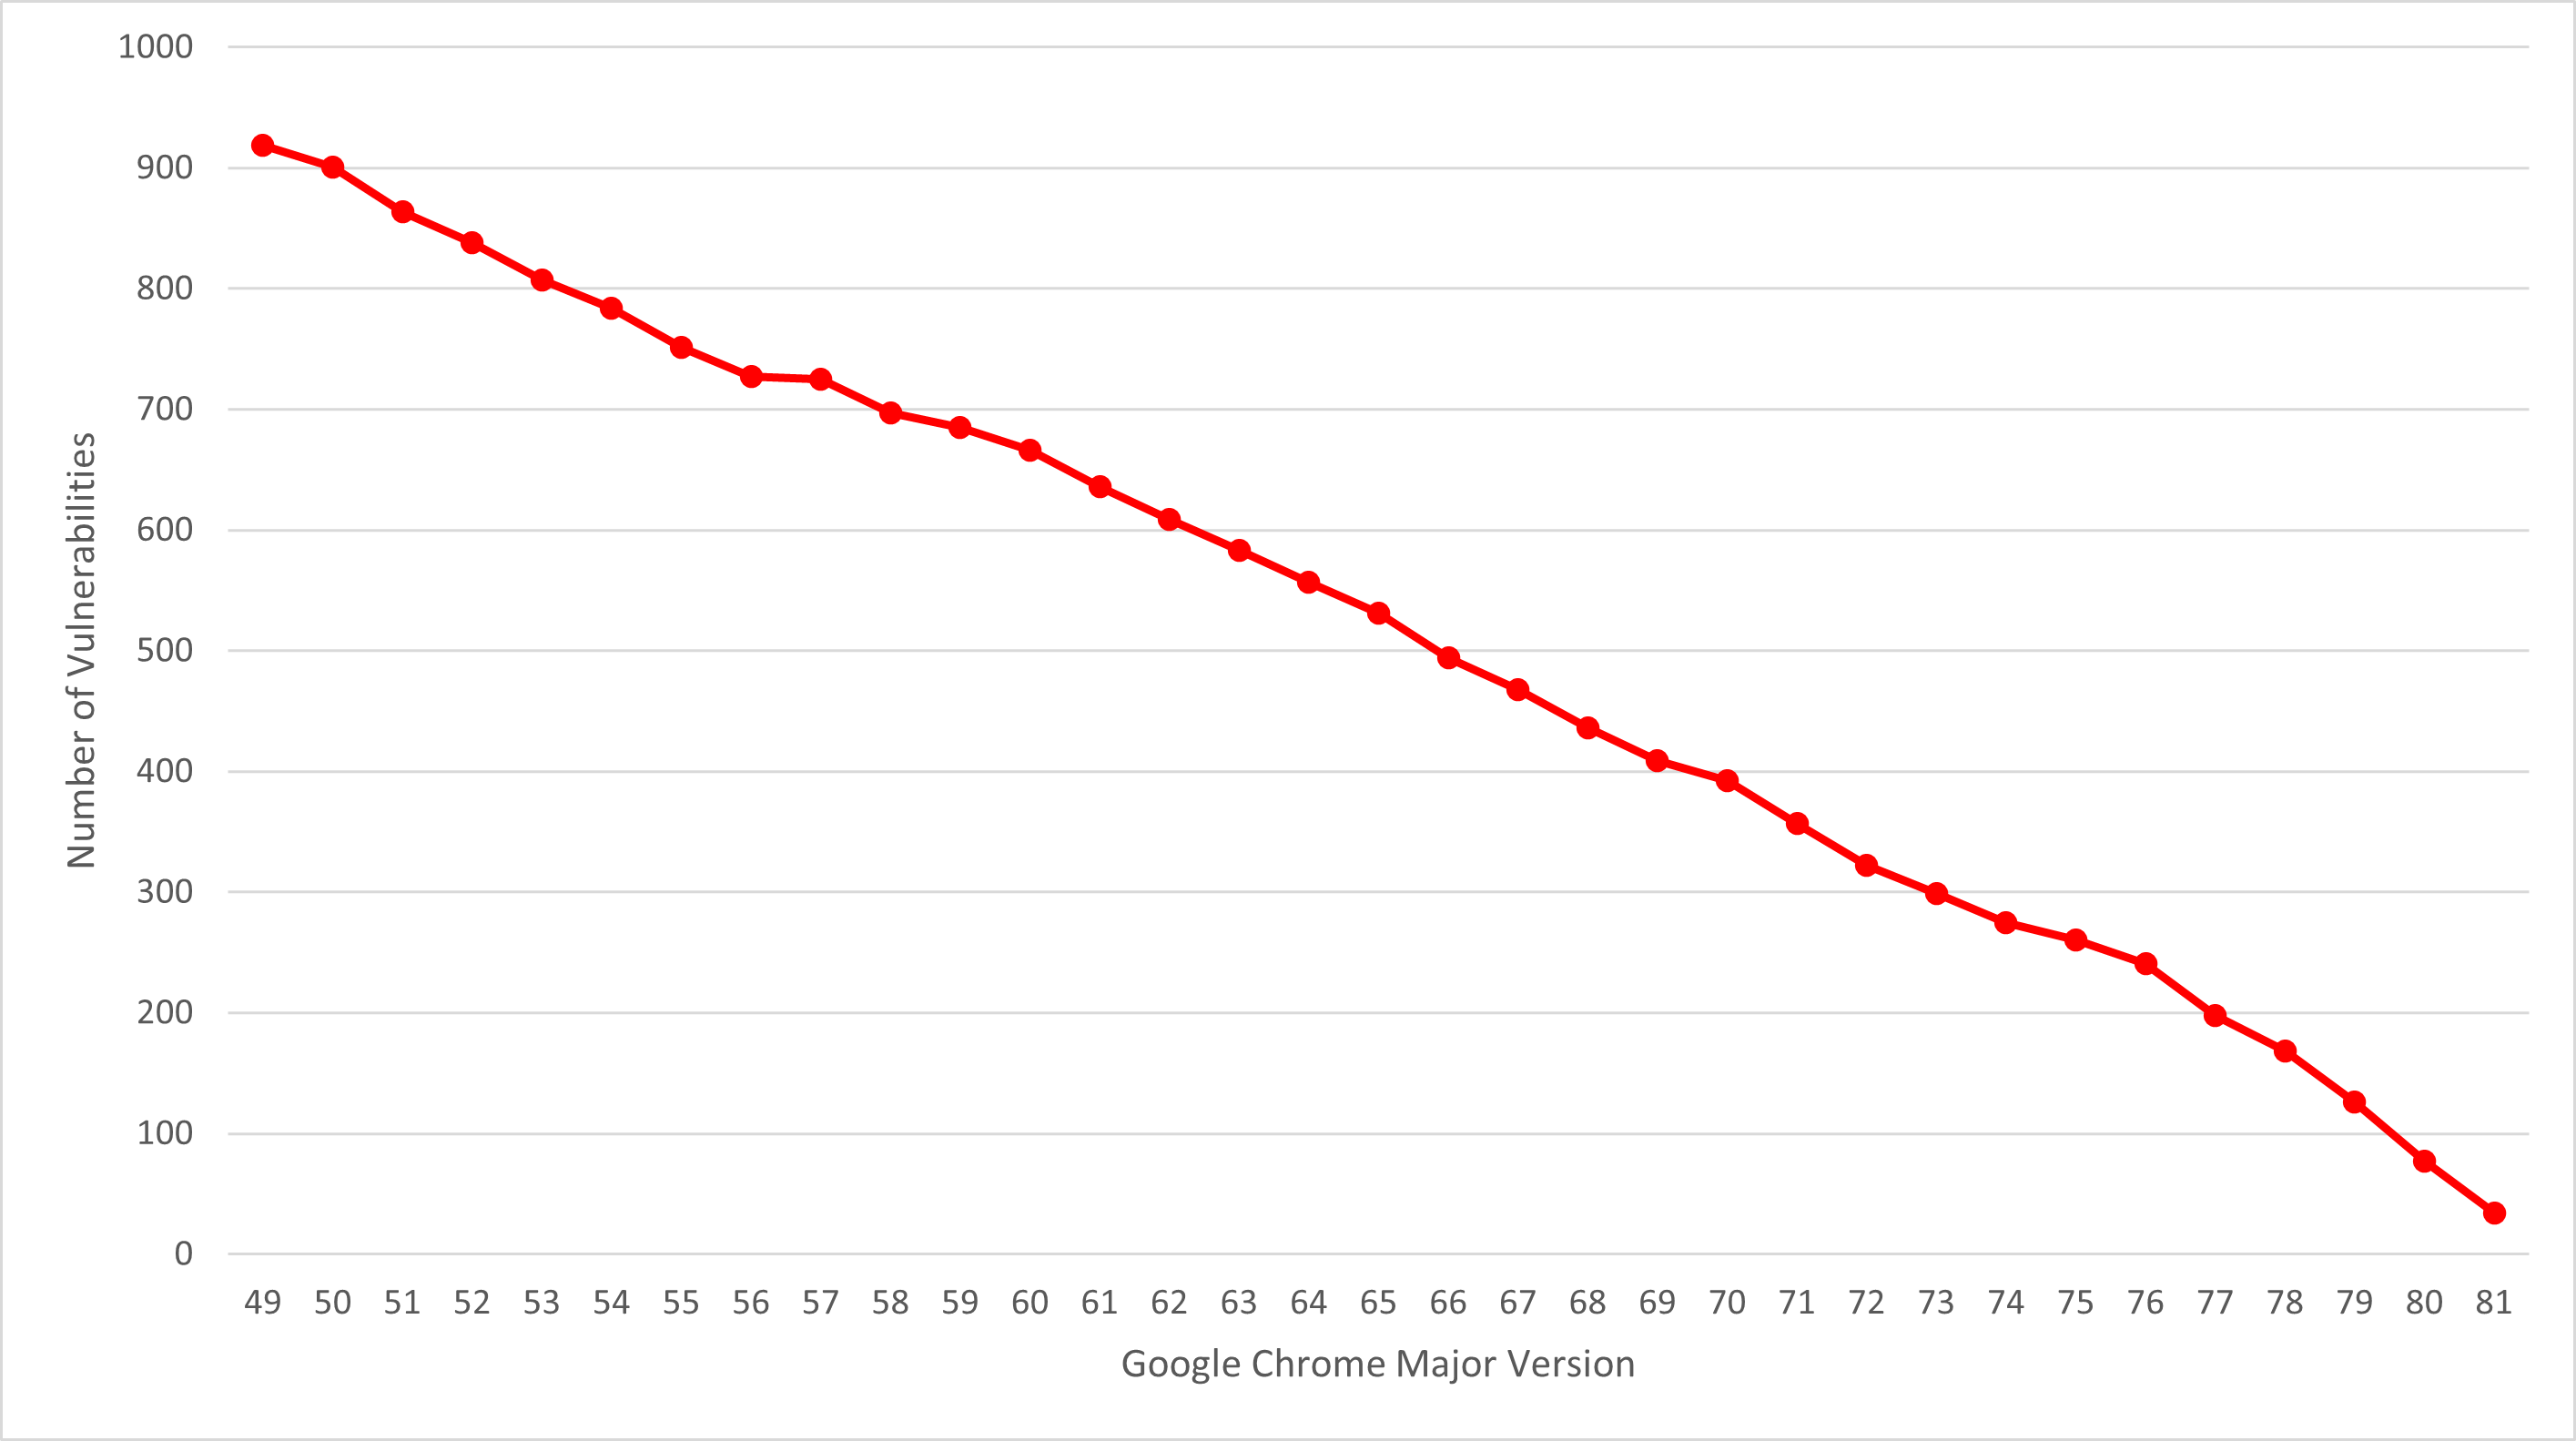
\includegraphics[width=\columnwidth]{figures/Chrome-Vulnerabilities.png}
    \caption{Google Chrome vulnerabilities per version.}
    \label{fig:chrome-vuln}
\end{figure}



\begin{figure}[ht]
    \centering
    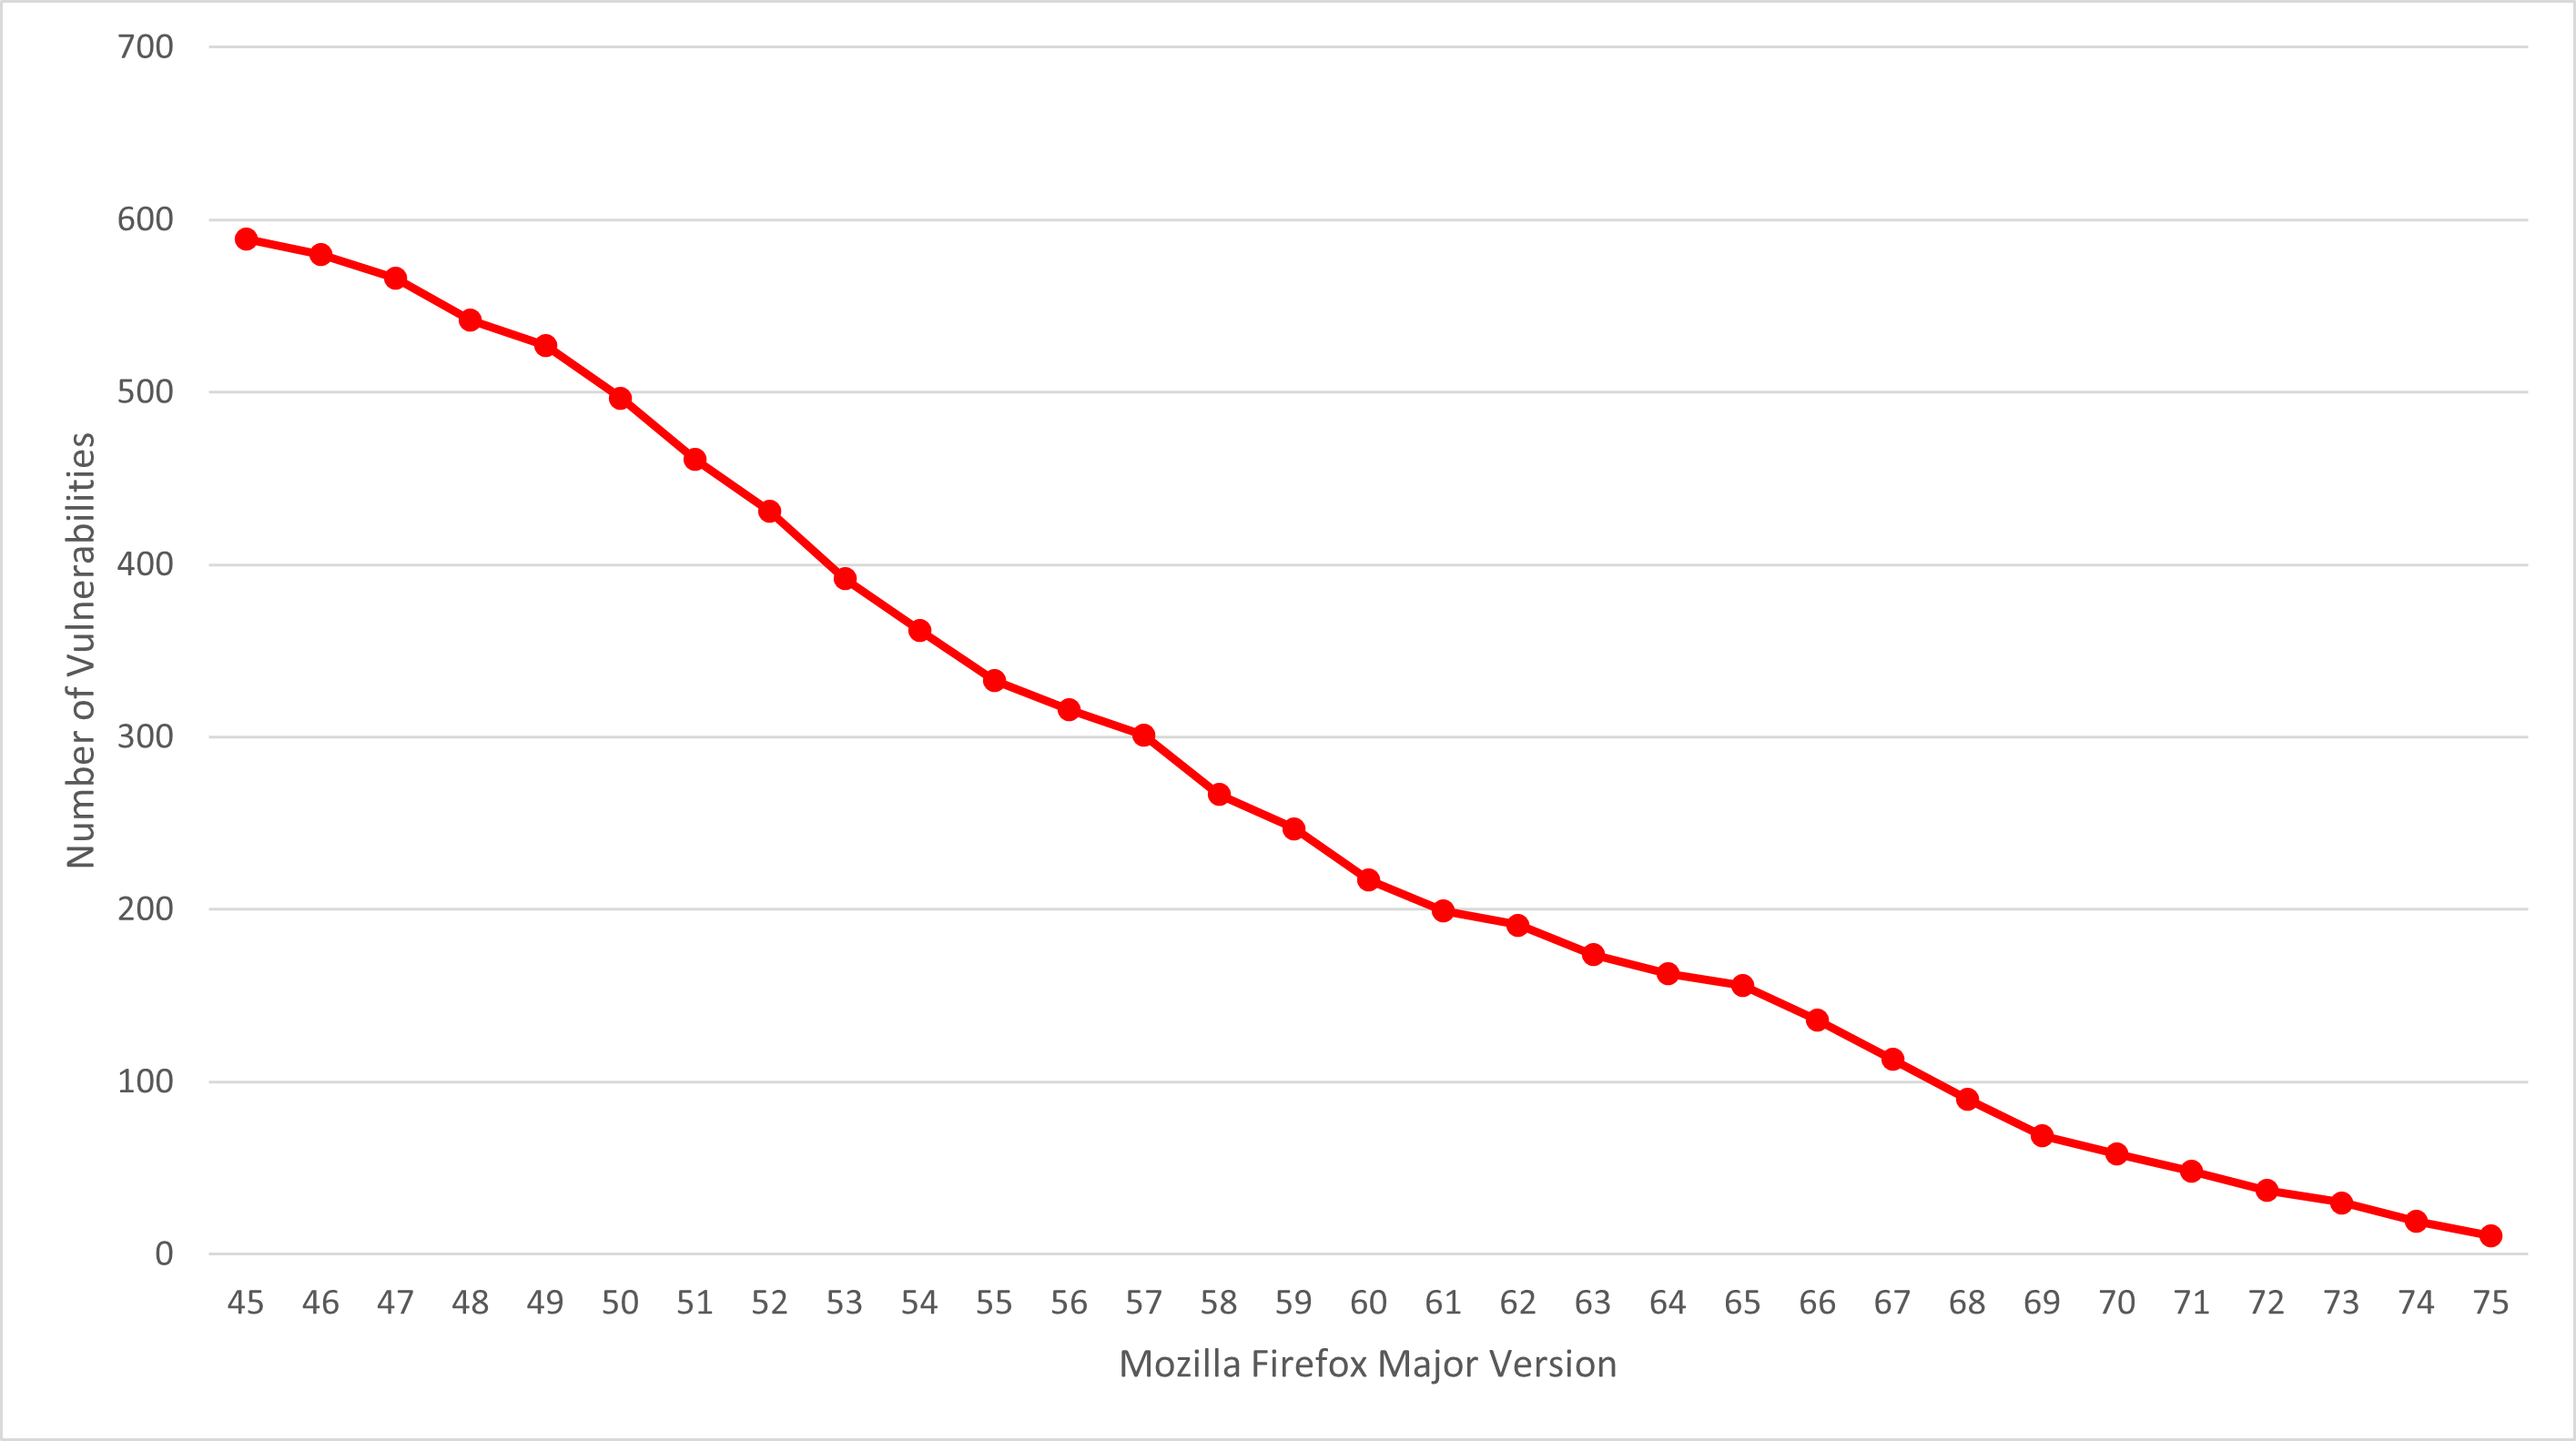
\includegraphics[width=\columnwidth]{figures/Firefox-Vulnerabilities.png}
    \caption{Mozilla Firefox vulnerabilities per version compared to features per version.}
    \label{fig:firefox-vuln}
\end{figure}

By comparing these two graphs with the graph in Figure \ref{featuretrends} we notice that number of features in a browser does not affect its number of vulnerabilities. Although browsers are having more and more features, they are have less reported vulnerabilities. This is completely different from what we expected. There may be two possible reasons for this finding. First, we could say that newer browsers are becoming more secure because vendors are patching previous security flaws in newer versions and newer versions do not contain previously reported vulnerabilities. In our idea, this is the main reason for these results. The other possible reason would be that there are still undetected vulnerabilities in newer features 

To summarize, we see that number of reported vulnerabilities in newer browser versions is rapidly decreasing which is totally in contrast with the increase in the number of features in newer browsers. So we could conclude that browsers are becoming more functional and more secure.